\documentclass[14pt]{beamer}
\mode<presentation>{}

\AtBeginSection[]{
\begin{frame}{Table of Contents}
	\tableofcontents[currentsection]
\end{frame}
}

\usepackage{xcolor}

% bibliography
\usepackage{natbib}

\title{Prospectus Defense}
\subtitle{The political determinants of FDI spillover and corruption}
\author{Anh Le}

\begin{document}

\begin{frame}
\titlepage
\end{frame}

\section{Motivation}

\begin{frame}
``One dollar from FDI is worth no more or less than one dollar of domestic investment'' -- Dani Rodrik
\end{frame}

\begin{frame}{\secname}
\begin{itemize}
\item<1->{FDI is important for growth because of its technological spillover}

\item<2-> 10\% increase in foreign presence = 9\% increase in local suppliers' productivity \citep{Havranek2011}
\end{itemize}
\end{frame}

\begin{frame}{\secname}
\begin{itemize}
\item<1-> But the effect is highly heterogeneous
\item<2-> \textcolor{red}{High spillover:} Taiwan (60s, 70s), Singapore (70s, 80s) electronics
\item<3-> \textcolor{red}{Low spillover:} Mexico, Costa Rica, Malaysia electronics
\end{itemize}
\end{frame}

\begin{frame}{\secname}
\begin{itemize}
\item<1-> Economic explanation: low absorptive capacity, weak financial institutions
\item<2-> But all of these are affected by policy, so where is the government?
\end{itemize}
\end{frame}

\begin{frame}{\secname: The government's role}
\begin{itemize}
\item<1-> Many works on institutions and \textit{quantity} of FDI \citep{Jensen2003, Li2003, Ahlquist2006}
\item<2-> Few works on politics and \textit{quality} of FDI
\end{itemize}
\end{frame}

\begin{frame}{\secname: The government's role}

\uncover<1->{
Voters / citizens probably do not care
\begin{itemize}
\item<1-> Low salience of trade policies even in highly affected groups \citep{Guisinger2009}
\end{itemize}
}


\uncover<2->{
If a policy area is not politicized, politicians' private benefits come into play
\begin{itemize}
\item<3-> A different approach from a sectoral \citep{Pandya2008} or a partisan \citep{Pinto2013} explanation
\end{itemize}
}
\end{frame}

\begin{frame}{\secname}
Thus, FDI spillover and corruption
\end{frame}

\section{Model}

\begin{frame}{\secname: choices}
\uncover<1->{One actor: the government official}

\uncover<2->{Choice over two-good bundle: spillover and private benefit}
\end{frame}

\begin{frame}{\secname: the constraint}

There is a trade off between \textit{spillover} and \textit{private benefit} because offering either cuts into the firm's profit
\begin{itemize}
\item<2-> Spillover: local content requirement
\item<3-> Private benefit: upfront cost and uncertainty cost 
\end{itemize}

... and the firm wants to maintain a minimum level of profit

\end{frame}

\begin{frame}{\secname: parameters of the constraint}
\uncover<1-> ``Price'' of spillover

\uncover<2->{``Price'' of private benefits}
\end{frame}

\begin{frame}{\secname: parameters of the constraint}
\begin{figure}
	\centering
    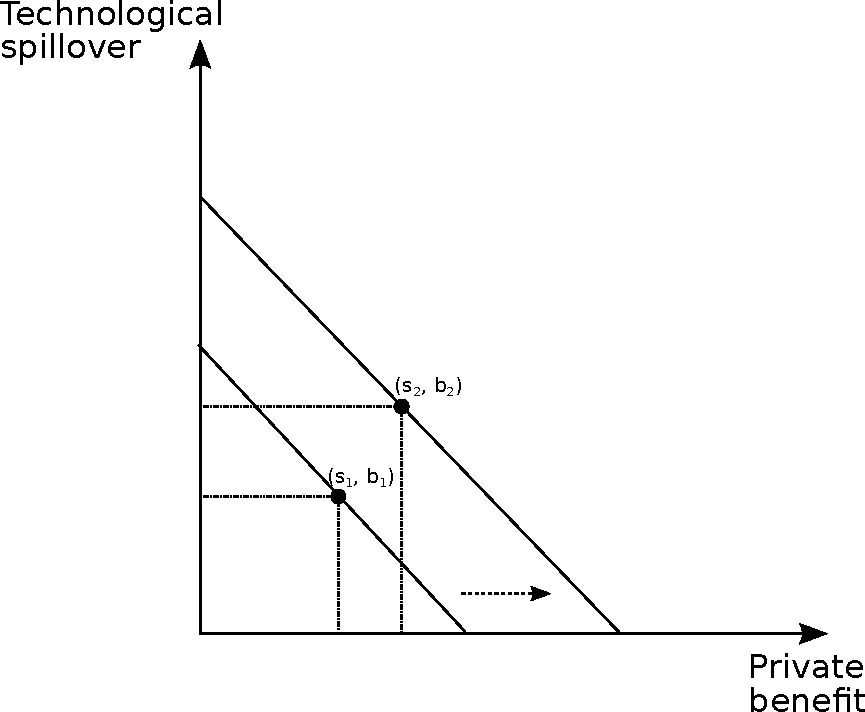
\includegraphics[width=0.75\textwidth, height=0.75\textheight,keepaspectratio]{../figure/budget_constraint}
    \label{fig:budget_constraint}
\end{figure}
\end{frame}

\begin{frame}{\secname: parameters of the constraint}
\begin{figure}
	\centering
    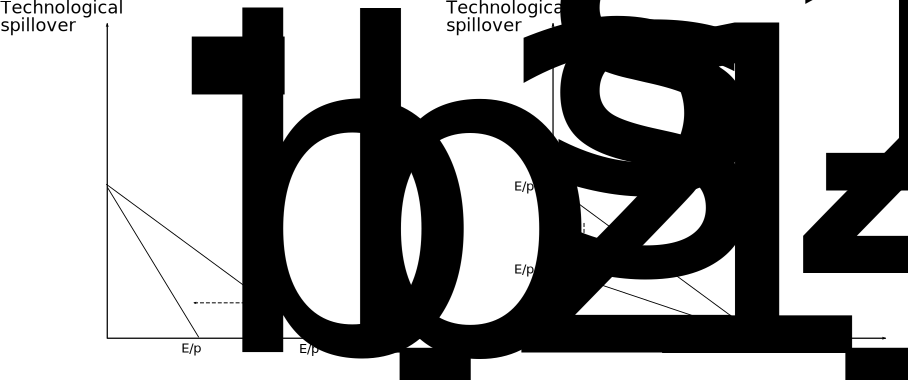
\includegraphics[width=\textwidth, height=\textheight,keepaspectratio]{../figure/absorptive_capacity}
    \label{fig:relative_price}
\end{figure}
\end{frame}

\begin{frame}{\secname: utility}
\begin{figure}
	\centering
    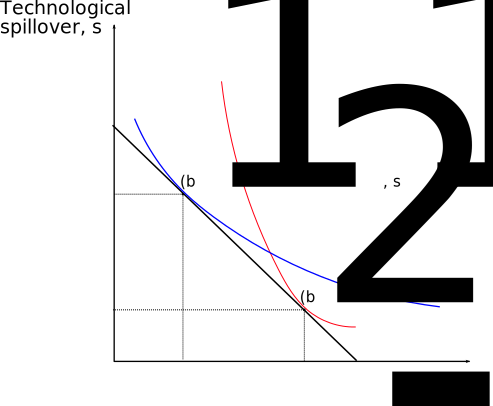
\includegraphics[width=0.75\textwidth, height=0.75\textheight,keepaspectratio]{../figure/indifference_curve}
    \label{fig:indifference_curve}
\end{figure}
\end{frame}

\begin{frame}{\secname: What are the assumptions?}
\begin{enumerate}
\item<1-> The firm only cares about its bottom line
\item<2-> The firm is profit satisficing.
\uncover<3->{(Can be relaxed in two-sided matching model)}
\end{enumerate}
\end{frame}

\section{Research Design}

\begin{frame}{Project 1---``price'' of spillover}
\begin{itemize}[<+->]
\item H: Officials extract spillover from firms with high potential for spillover and get bribes from the others
\item Empirical strategy: Instrument for \textit{spillover potential}
\begin{itemize}[<+->]
\item Spillover in US industries as instrument: the weak instrument issue is there but can be tested
\item Question: Data from any other country that can be used to estimate spillover?
\end{itemize}
\end{itemize}
\end{frame}

\begin{frame}{Project 2---``price'' of private benefits}
\begin{itemize}
\item<1-> H: Officials extract bribes from firms for whom it costs less to bribe
\item<2-> Empirical strategy: OECD anti-bribery convention as an exogenous shock to the price of bribes (diff-in-diff)
\end{itemize}
\end{frame}

\begin{frame}{Project 3---the official's utility function}
\begin{itemize}
\item<1-> H: Officials with a short time horizon prefers private benefits over bribe
\item<2-> Empirical strategy: term-limit for Vietnamese provincial official (RDD)
\end{itemize}
\end{frame}

\begin{frame}{Project 4---two-sided logit matching}
\begin{itemize}
\item<1-> H: Officials with a short time horizon prefers private benefits over bribe
\item<2-> Empirical strategy: two-sided logit
\end{itemize}
\end{frame}

\begin{frame}{Project 4---two-sided logit matching}
\begin{itemize}[<+->]
\item A many (firms)-to-one (country) matching problem
\item Goal: Estimate the preference of firms and officials regarding one another's traits
\item Data: a random sample of firms and where they invest
\item Expectation Maximization algorithm to fill in the unobserved investment offer
\item Question: BEA requires citizenship. Any other data?
\end{itemize}
\end{frame}

\begin{frame}
\footnotesize
\bibliographystyle{chicago}
\bibliography{library}
\end{frame}


\end{document}